
%(BEGIN_QUESTION)
% Copyright 2010, Tony R. Kuphaldt, released under the Creative Commons Attribution License (v 1.0)
% This means you may do almost anything with this work of mine, so long as you give me proper credit

Suppose we have an Allen-Bradley MicroLogix 1000 PLC connected to three momentary-contact pushbutton switches as shown in this illustration:

$$\includegraphics[width=15.5cm]{i04685x01.eps}$$

Determine the bit statuses of {\tt I:0/0}, {\tt I:0/1}, and {\tt I:0/3} when switch A is pressed, switch B is unpressed (released), and switch C is pressed.

\underbar{file i04685}
%(END_QUESTION)





%(BEGIN_ANSWER)

Bit statuses:

\begin{itemize}
\item{} {\tt I:0/0} = 0
\item{} {\tt I:0/1} = 0
\item{} {\tt I:0/3} = 1
\end{itemize}

%(END_ANSWER)





%(BEGIN_NOTES)


%INDEX% PLC, relating I/O status to virtual elements 

%(END_NOTES)


